\chapter{Implementation}
\label{chap:implementation}
This chapter presents the implementation of the proposed methodology outlined
in chapter~\ref{chap:methodology}. It demonstrates the feasibility of using Active Inference (AIF) to dynamically manage elasticity in distributed edge pipelines while upholding Service Level Objectives (SLOs). A Python-based prototype simulates a real-time video processing system and compares the AIF agent to baseline control strategies under constrained edge conditions.

The prototype of the distributed pipeline and the experimental results are available in a publicly accessible repository \footnote{The prototype of the stream processing framework is available at \href{https://github.com/JohnnyElaine/bsc_aif_parallel_pipeline}{GitHub}, accessed on July 22nd 2025.}.


The prototype implements a parallel and distributed processing pipeline inspired by Apache Flink~\cite{carbone_apache_2015}. It processes video streams using YOLOv11 inference and dynamically controls elasticity via an AIF agent deployed at the producer.

\section{System Architecture}
The architecture consists of three roles:
\begin{itemize}
    \item \textbf{Producer:} Splits the frames of the video stream into tasks, and dispatches them to workers. It also acts as the central controller of elasticity and exposes control of the \textit{stream quality parameters} to its AIF agent.
    \item \textbf{Workers:} Execute YOLOv11 inference on received tasks and sends the result to the Collector.
    \item \textbf{Collector:} Aggregates processed results into an ordered output stream.
\end{itemize}

Communication is fully asynchronous and implemented using ZeroMQ sockets~\cite{noauthor_zeromqpyzmq_nodate}. Task dispatch from the Producer to Workers uses the REQ-ROUTER pattern, forming a pull-based work distribution model, also known as a Load-Balancing Pattern. Processed results are forwarded from Workers to the Collector using the PUSH-PULL pattern. This design ensures that work is allocated based on each worker’s readiness, optimizing system responsiveness and throughput.

ZeroMQ sockets are multiplexed using event loops, allowing simultaneous listening and sending. Task payloads (NumPy arrays) are transmitted as raw binary data without any copying, by leveraging the buffer interface they implement. Task metadata is serialized using msgpack \cite{noauthor_msgpackmsgpack-python_nodate} for compact binary transport.


\section{Producer Architecture}
The producer fulfills three roles: task generation, elasticity control, and agent orchestration.

\subsection{Task Queue and Generation}
A continuous stream of video frames is segmented into tasks and temporarily stored in a FIFO queue. Each \texttt{Task} includes:
\begin{itemize}
    \item \texttt{type:} Task purpose (e.g., INFERENCE, COLLECT).
    \item \texttt{id:} Unique identifier.
    \item \texttt{stream\_key:} Identifier for multi-stream support.
    \item \texttt{data:} A video frame, as a NumPy \texttt{ndarray}.
\end{itemize}
The number of tasks generated per second is dependent on the current configuration of the \textit{fps} parameter. Tasks are served upon worker request and consumed from the queue.

\subsection{Service Level Objectives}

Table~\ref{tab:slo-table} shows 4 types of SLOs intending to guarantee the QoE. These SLOs serve as constraints that guide the elastic adaptation process of the producer, helping to maintain a balance between processing quality and system stability.

\begin{table}[h]
    \centering
    \begin{tabular}{@{}lll@{}}
        \toprule
        \textbf{Var.} & \textbf{Rel.} & \textbf{Description} \\
        \midrule
        \textit{memory usage} 
            & \( \leq \theta_\text{mem} \) 
            & container memory usage \\
            
        \textit{task queue size} 
            & \( \leq \textit{fps} \cdot \varepsilon_\text{queue} \) 
            & task queue size \\
            
        \textit{avg process time} 
            & \( \leq \frac{1}{\textit{fps}} \cdot \varepsilon_\text{global}\) 
            & average global processing time \\
            
        \textit{highest avg process time} 
            & \( \leq \frac{1}{\textit{fps}} \cdot \varepsilon_\text{worker}\) 
            & worker with the highest average processing time \\
        \bottomrule
    \end{tabular}
    \caption{Service Level Objectives (SLOs) at the producer}
    \label{tab:slo-table}
\end{table}


The \textbf{Memory Usage SLO} ensures that the container does not exceed a specified memory capacity \(\theta_\text{mem}\). This protects the system from memory saturation, which would cause severe performance degradation as tasks might be offloaded to slower storage or dropped entirely.

\paragraph{Task Queue Size SLO}
Ensures that the number of unprocessed tasks remains within a reasonable limit, based on the current \textit{fps} parameter and a tolerance \(\varepsilon_\text{queue}\). A growing queue indicates that the processing capacity of the workers is insufficient for the current workload. This SLO acts as a safeguard for maintaining real-time responsiveness. The tolerance threshold must be set low enough to avoid the accumulation of multiple seconds worth of unprocessed frames in the task queue. At the same time, it must be sufficiently permissive to prevent immediate reactions to minor fluctuations, such as transient network delays. Based on empirical evaluation, a recommended tolerance range for the queue size SLO is \( 2 \geq \varepsilon_\text{queue} \geq 4\).

\paragraph{Average Global Task Processing Time SLO} Ensures that, on average, all workers combined can keep pace with the input stream. It is computed by tracking the processing time of the most recent \(n\) completed tasks using a moving average window. These statistics are reported by each worker during regular task requests. The goal is to ensure that the cumulative system throughput is sufficient to maintain real-time responsiveness. \(\varepsilon_\text{global}\) denotes a tolerance factor. A recommended value is \(\varepsilon_\text{global} = 1\), meaning the average time to process a single task must not exceed the current task generation time interval. Violations of this SLO indicate that the aggregate compute capacity of the system is insufficient to sustain the current input rate. This SLO serves as a holistic throughput constraint, ensuring that the pipeline as a whole can process frames as quickly as they arrive.

Violations of this SLO indicate that the aggregate compute capacity of the system is insufficient to sustain the current input rate. This SLO serves as a holistic throughput constraint, ensuring that the pipeline as a whole can process frames as quickly as they arrive.

\paragraph{Highest Per-Worker Average Task Processing Time SLO} Enforces an upper bound on the slowest worker’s performance. It ensures that no individual worker lags so far behind that its results become irrelevant to the output stream. This is particularly important in distributed pipelines, where late-arriving results may be discarded if the collector has already progressed past the corresponding task ID.

Here, \(\varepsilon_\text{worker} \geq 1\) provides additional tolerance compared to the global SLO. A typical setting is \(\varepsilon_\text{worker} = 4\), allowing slower nodes to process a task in up to 4 times the time budget permitted by the frame rate. By ensuring that even the slowest node performs within tolerable bounds, the system can maintain temporal coherence and avoid dropping results from late workers.

\subsection{SLO State Discretization}
To enable discrete decision-making within the Active Inference controller, the continuous \textit{SLO value} is transformed into one of three discrete SLO states:

\begin{table}[h]
    \centering
    \begin{tabular}{@{}lll@{}}
        \toprule
        \textbf{SLO State} & \textbf{SLO Value} & \textbf{Description} \\
        \midrule
        OK        & \( x < 0.8 \)                          & Constraint is comfortably fulfilled \\
        WARNING   & \( 0.8 \leq x \leq 1.0 \)             & Constraint is nearing violation     \\
        CRITICAL  & \( x > 1.0 \)                         & Constraint is violated              \\
        \bottomrule
    \end{tabular}
    \caption{Discretization of SLO values into discrete system states.}
    \label{tab:slo-states}
\end{table}


This ternary discretization introduces a minimal yet effective abstraction over the continuous SLO domain. It enables the Active Inference agent to reason over discrete system states when selecting actions. OK states reflect a healthy operating condition; WARNING states indicate a need for caution and CRITICAL states signal a SLO violation.


\subsection{Elasticity and Stream Parameter Control}
The \textit{Producer} serves as the central control entity for elasticity. It continuously monitors and adjusts three key \textit{quality parameters} of the video stream: (1) frames per second (\textit{fps}), (2) \textit{resolution}, and (3) \textit{inference quality}. While the producer directly sets fps and resolution by modulating task generation frequency and resizing video frames, inference quality refers to the YOLOv11 model variant employed by the worker nodes, e.g., \texttt{LOW} $\rightarrow$ \texttt{YOLOv11n}, \texttt{MEDIUM} $\rightarrow$ \texttt{YOLOv11s}, \texttt{HIGH} $\rightarrow$ \texttt{YOLOv11m}.

Although inference is executed on the workers, the producer dictates the inference quality of the entire system. To enforce a configuration change, it maintains a dedicated \textit{backlog} for each worker node. When the producer initiates a change (e.g., \texttt{MEDIUM} $\rightarrow$ \texttt{LOW}), it inserts the entry \texttt{CHANGE\_INFERENCE\_QUALITY=LOW} into the backlog of every registered worker. Upon the next task request, the worker's backlog is evaluated. If a configuration change is pending, the producer replies with a message of type \texttt{CHANGE} detailing all configuration changes the worker needs to make. This includes \texttt{CHANGE\_INFERENCE\_QUALITY=LOW}, instructing the worker to adapt its local inference model accordingly. Once the change is applied, the worker resumes normal task processing.

This design ensures that all nodes operate under a globally consistent inference configuration while minimizing coordination overhead.

\subsection{Active Inference Agent}
\label{sec:evaluation-implementation-active-infernce-agemt}
The control of the \textit{quality parameters} is delegated to the AIF agent running on the producer. Its objective is to uphold all defined Service Level Objectives (SLOs) while maximizing the Quality of Experience (QoE) through adaptive control of frame rate (FPS), resolution, and inference quality. The agent is implemented using pymdp \cite{heins_pymdp_2022} and operates continuously, executing one action-perception cycle every 500\,ms. Each cycle results in no action or a change in \textit{stream quality parameters}. 

\paragraph{Generative Model Construction.}
The agent operates a \textit{generative model} comprising the following components:
\begin{itemize}
  \item \textbf{Observation model \(P(o \mid s)\):} SLO values and quality parameters
  \item \textbf{Transition model \(P(s_{t+1} \mid s_t,a_t)\):} Latent configuration state
  \item \textbf{Prior preferences over observations \(P(o)\):} Strong preference for high quality parameters and equally strong aversion for SLO violations
  \item \textbf{Prior beliefs about hidden states \(P(s_0)\):} Inital quality parameter configuration.
\end{itemize}

\paragraph{Discrete State and Action Space Construction.}
Each configuration of the system is represented as a tuple of discrete quality parameter values:
\begin{itemize}
  \item \textbf{Resolution} $\in \{$480p, 720p, 1080p$\}$
  \item \textbf{Frame Rate (FPS)} $\in \{$10, 15, 20, 25, 30$\}$
  \item \textbf{Inference Quality} $\in \{$LOW, MEDIUM, HIGH$\}$
\end{itemize}

\paragraph{Actions}
The AIF agent operates using a \textit{relative control} strategy. Rather than selecting absolute parameter values, each action proposes an incremental change along one of the quality parameter dimensions. Specifically, the agent can:

\begin{itemize}
  \item \textbf{Frame Rate (FPS):} increase, decrease, or retain the current FPS setting.
  \item \textbf{Resolution:} increase, decrease, or retain the current resolution setting.
  \item \textbf{Inference Quality:} increase, decrease, or retain the YOLOv11 model quality.
\end{itemize}

A full action is a tuple $(a_\text{res}, a_\text{fps}, a_\text{qual})$, representing a joint change in the current configuration.


This results in an action space of $3 \times 3 \times 3 = 27$ discrete joint actions. Each action tuple $(\Delta_\text{res}, \Delta_\text{fps}, \Delta_\text{qual})$ specifies a directional adjustment in each dimension, where \(\Delta \in \{-1, 0, +1\}\). The current configuration is then updated accordingly, subject to parameter bounds. For instance, an action with \(\Delta_\text{fps} = -1\) reduces the frame rate by one level (e.g., from 30 to 25 FPS), unless the lower bound is already reached.

This relative formulation reduces the complexity of the policy space while enabling fine-grained and adaptive parameter control over time.

\paragraph{Online Model Learning.}
To adapt to non-stationary runtime conditions, the agent continuously refines its internal model during operation. This is achieved via the following update steps executed at each cycle:

\begin{itemize}
  \item \texttt{agent.update\_A(\(o_t\)):} Updates the observation model \( P(o \mid s) \) using the newly observed data.
  \item \texttt{agent.update\_B(\(Q(s_t)\)):} Updates the transition model \( P(s_{t+1} \mid s_t, a_t) \) based on the posterior belief \(Q(s_{t})\) from the previous timestep.
\end{itemize}

This learning mechanism allows the agent to gradually internalize the causal structure of the environment, e.g., how a reduction in resolution affects memory usage or how inference quality relates to task processing time. As a result, the agent becomes increasingly adept at selecting configurations that uphold SLOs under varying conditions.

\paragraph{Decision Prioritization and Trade-offs.}
The agent’s decision-making is shaped by its preference structure. Violations of any SLO are assigned a utility penalty large enough to outweigh the benefit of increasing QoE. This lexicographic structure ensures that:
\begin{itemize}
  \item SLO violations are strictly avoided whenever possible.
  \item QoE is maximized only within the bounds of safe operation.
\end{itemize}

In effect, the agent internalizes a dynamic control policy that minimizes long-term surprise~\cite{sedlak_adaptive_2024}, adapts to the environment via learning, and maintains operational stability under edge constraints.


\section{Worker Architecture}
\label{sec:implementation-worker-architecture}
Worker nodes form the computational core of the distributed pipeline. Their role is to execute inference tasks on data segments received from the producer and transmit the results to the collector. Each worker operates independently and adheres to a pull-based communication model, thereby ensuring a decentralized and scalable architecture.

Crucially, workers do not maintain internal logic for deciding whether a parameter change is required. Instead, they execute the received task exactly as instructed. If a message with type \texttt{CHANGE} is received, the worker applies all changes listed in the message's metadata—such as switching the YOLOv11 model or updating FPS/resolution targets—and then resumes regular processing. This design simplifies the worker logic and ensures synchronization across the system with minimal overhead.

\begin{figure}[htbp]
    \centering
    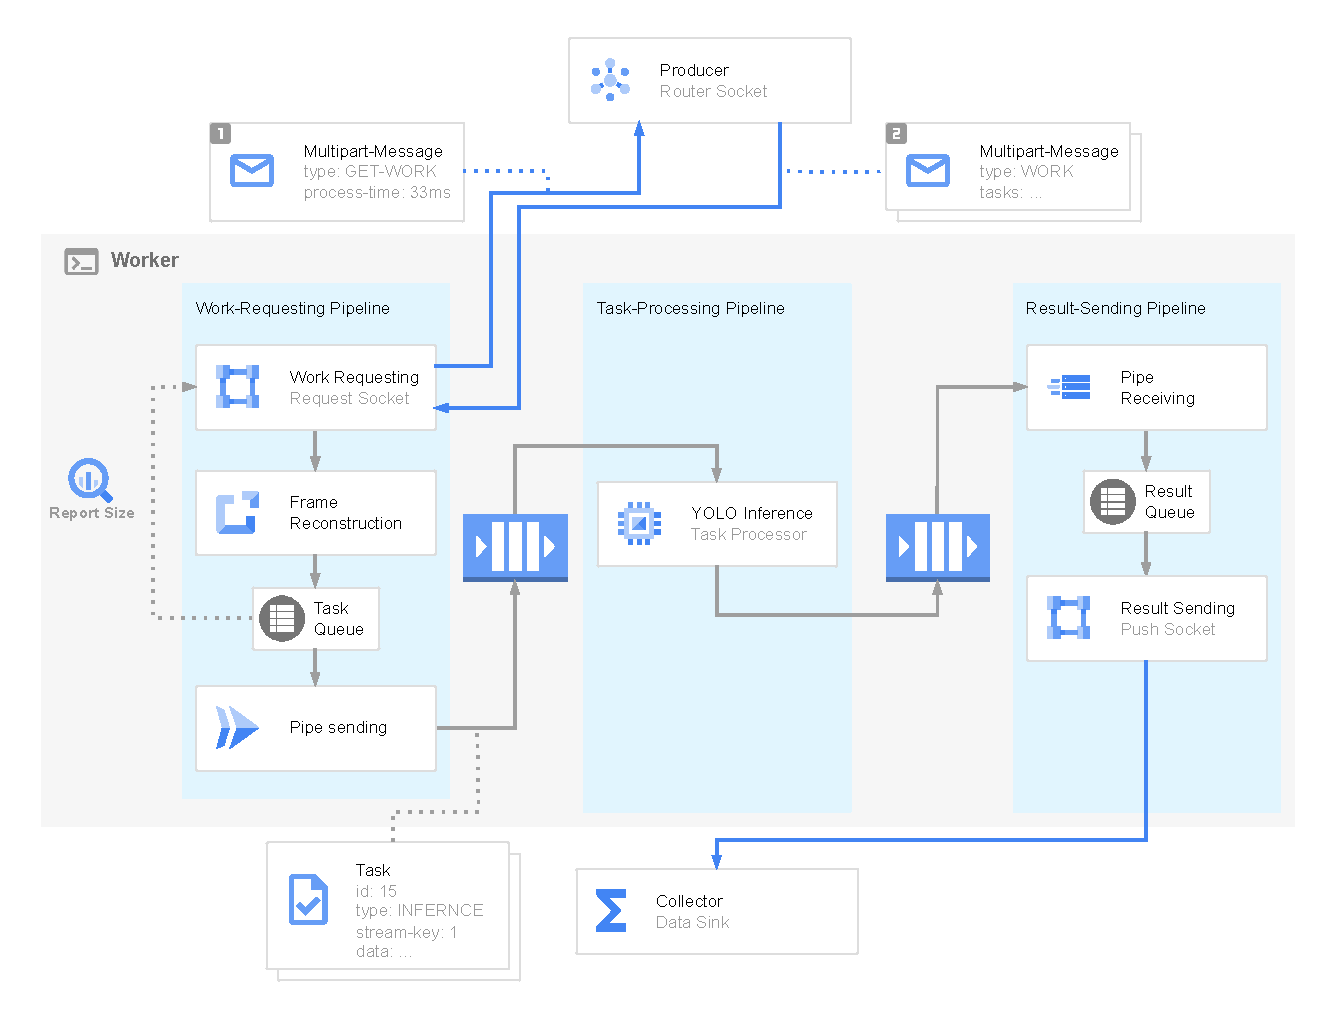
\includegraphics[width=\textwidth]{img/implementation/implementation_worker_architecture.drawio.pdf}
    \caption{Worker architecture. Detailing the process of requesting tasks, processing them, and sending the results to the collector}
    \label{fig:implementation-worker-architecture}
\end{figure}

\subsection{Startup and Registration}
Upon initialization, a worker registers with the producer using its unique identifier and receives the current stream configuration, including the active inference quality settings. The worker then initializes the YOLO models for future inference.

\subsection{3 Process Architecture}
To support concurrent operations and avoid resource contention, each worker is structured into three pipelines, each implemented as an independent process. This modular design enables clean separation of responsibilities and optimizes throughput by decoupling I/O-bound and compute-bound operations.

Most importantly, the use of three separate processes allows the worker to avoid bottlenecks caused by Python’s GIL and to exploit multicore CPUs effectively.

\subsection{Work Requesting Pipeline.}
This pipeline manages interaction with the producer and forwards received tasks for processing. It sends requests to the producer using a ZeroMQ REQ socket to request work. 

Each time the worker requests a new task, it attaches its most recent processing time to the request. This metric is used by the producer to compute both global and per-worker SLOs. By making performance reporting part of the task request cycle, the system avoids the need for separate monitoring channels and maintains low overhead.

Received tasks are buffered until they are ready to be handed over to the \textit{processing pipeline}. New work is requested whenever the task buffer is empty. If the producer facilitates a change in the worker's configuration and the worker receives a message with \texttt{type=CHANGE}, it immediately implements all changes detailed within the message. For example, switching YOLOv11 model.

\subsection{Processing Pipeline}
This process is dedicated to executing inference on received tasks. Upon receiving a task from the \textit{work requesting pipeline} with \texttt{type=INFERENCE}, it processes the tasks by executing inference using the currently active YOLOv11 model. The result is then re-packaged into a new task with \texttt{type=COLLECT} and forwarded to the \textit{result sending pipeline}.

\subsection{Result Sending Pipeline.}
This pipeline handles the transmission of processed results to the collector. It receives results from the \textit{processing pipeline} and enqueues them for transmission. Once ready, the results are then pushed to the collector.

\section{Collector Architecture}
The collector node forms the terminal stage of the distributed pipeline. Its primary responsibility is to receive results from worker nodes, reconstruct the output stream in the correct order, and optionally render or store the final output. 


\subsection{Result reordering}
The collector receives completed tasks from workers via a ZeroMQ PULL socket. Each task includes a unique \texttt{id} and a \texttt{stream\_key}, which together uniquely identify a specific frame within a logical stream. To maintain correct ordering, the collector uses a blocking dictionary that buffers out-of-order results until all preceding frames have arrived. If a task is delayed or lost—for example, due to a slow or faulty worker—it is dropped after a configurable timeout using a strike-based policy, thereby preserving the responsiveness of the system.

\subsection{Support for Concurrent Streams}
The architecture supports multiple concurrent data streams by tracking and assembling frames independently based on the \texttt{stream\_key} attribute. This is particularly important for the evaluation scenario involving changing workload, where multiple video streams are processed in parallel. Each stream is assigned its own logical ordering buffer, and the collector ensures that results from different streams do not interfere with one another.

The problem of stream reordering under asynchronous and heterogeneous compute conditions is well known in distributed systems. Apache Flink, for example, uses watermarks and checkpoint barriers to achieve consistent stream processing under variable network and compute latencies~\cite{carbone_apache_2015}. The collector in this prototype adopts a simplified design that reflects these core principles while remaining lightweight and suitable for resource-constrained edge deployments.